\PassOptionsToPackage{brazil,american}{babel}
\documentclass[12pt]{article}

\usepackage{sbc-template}
\usepackage[brazil,american]{babel}
\usepackage[utf8]{inputenc}

\usepackage{graphicx}
\usepackage{url}
\usepackage{float}
\usepackage{listings}	
\usepackage{color}
\usepackage{todonotes}
\usepackage{algorithmic}
\usepackage{algorithm}
\usepackage{hyperref}
     
\sloppy

\title{Experimento 7\\ 
	Implementação de Circuitos Combinacionais com Multiplexadores}

\author{
	Lucas Mafra Chagas, 12/0126443 \\
	Marcelo Giordano Martins Costa de Oliveira,  12/0037301
}


\address{Dep. Ciência da Computação -- Universidade de Brasília (UnB)\\
	CiC 116351 - Circuistos Digitais - Turma C
	\email{\{giordano.marcelo, chagas.lucas.mafra\}@gmail.com}
}

\begin{document} 

\maketitle

 \begin{abstract}
	 In this experiment, we focus on building combinational circuits using Multiplexers.
 \end{abstract}  
 \begin{resumo} 
	O foco desse experimento é construir Circuitos Combinacionais utilizando Multiplexadores.
 \end{resumo}
\section{Objetivos}
\label{sec:Objetivos}

O objetivo deste experimento é adquirir conhecimento na implementação e também utilização de multiplexadores, que são circuitos combinacionais.

\section{Materiais} 
\label{sec:Materiais}

\begin{itemize}						 							
    \item Painel Digital
 
    \item \textit{protoboard}
    
    \item Fios conectores
    
    \item Portas Lógicas NAND e NOT
    
	\item 2 x MUX-4
	
	\item DECOD-16
    
\end{itemize}


\section{Introdução}
\label{sec:Introducao}
\subsection{Multiplexadores e Demultiplexadores}
Um multiplexador é um circuito combinacional lógico projetado que tem como saída única e compartilhada um e somente um de seus inputs de dados, a partir da aplicação de um sinal de controle. O demultiplexador, por sua vez, realiza a operação inversa.

\begin{figure}[H]
	\centering
	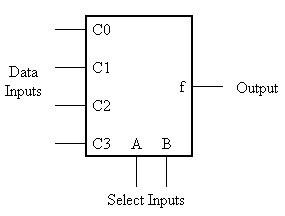
\includegraphics[width=.5\textwidth]{estrmux.png}
	\caption{Estrutura de um Multiplexador}
	\label{fig:estmux}
\end{figure}

Sob o ponto de vista da implementação de seus circuitos, os multiplexadores e demultiplexadores são simplesmente circuitos combinacionais com diversas entradas e somente uma saída, ou vice-versa.

\begin{figure}[H]
	\centering
	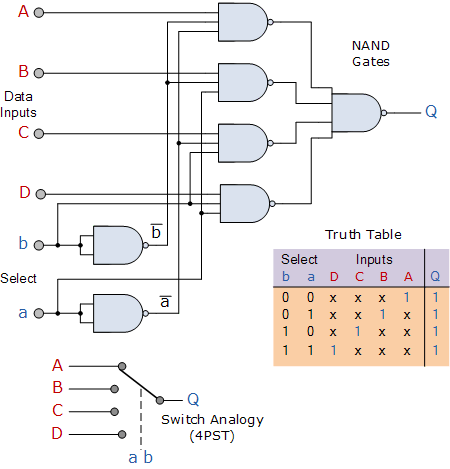
\includegraphics[width=.5\textwidth]{muxedemux.png}
	\caption{Implementação de um multiplexador com 7 portas NAND`s}
	\label{fig:muxedemux}
\end{figure}

\subsection{Aplicações}
	A eficiência dos sistemas de comunicação pode ser consideravelmente aumentada ao utilizar-se multiplexadores, por permitir a transmissão de diferentes tipos de dados (como áudio e vídeo) ao mesmo tempo, usando uma única linha de transmissão. Eles também são utilizados para implementar grandes quantidades de memória no computador, reduzindo drasticamente a quantidade de fios de cobre necessários para ligar conectar a memória a outras partes do circuito. Isso se deve ao fato de um multiplexador ser capaz de implementar qualquer função booleana genérica. Quando temos uma função em que obter a tabela verdade não é tão simples, a utilização de multiplexadores e demultiplexadores pode simplificar o problema da implementação dessa função.
	
\section{Procedimentos}
\label{sec:Procedimentos}

\subsection{Usar um MUX - 4 duplo em MSI para implementar um somador completo}
\label{sec:Mux}

Para um somador completo, temos que considerar as entradas A,B e C, com A e B sendo os bits na qual se quer somar e C sendo o carry vindo da soma anterior. Como saídas temos que considerar T e S, com S sendo o valor da soma dos 3 bits de entrada e T sendo o carry gerado por essa soma.	Temos portanto, que a tabela verdade para esse circuito seria:

\begin{figure}[H]
\centering
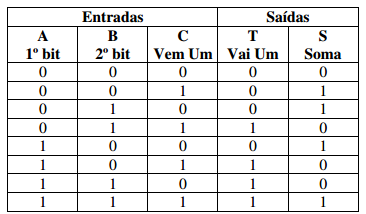
\includegraphics[width=.5\textwidth]{tvsc.png}
\caption{Tabela verdade de um Somador Completo}
\label{fig:tvsc}
\end{figure}

Utilizando a tabela na Figura 5 como refrência e tendo em mente que o circuito deveria ser montado a partir de um MUX - 4 duplo, o seguinte esquema para o circuito a ser implementado foi projetado:

\begin{figure}[H]
	\centering
	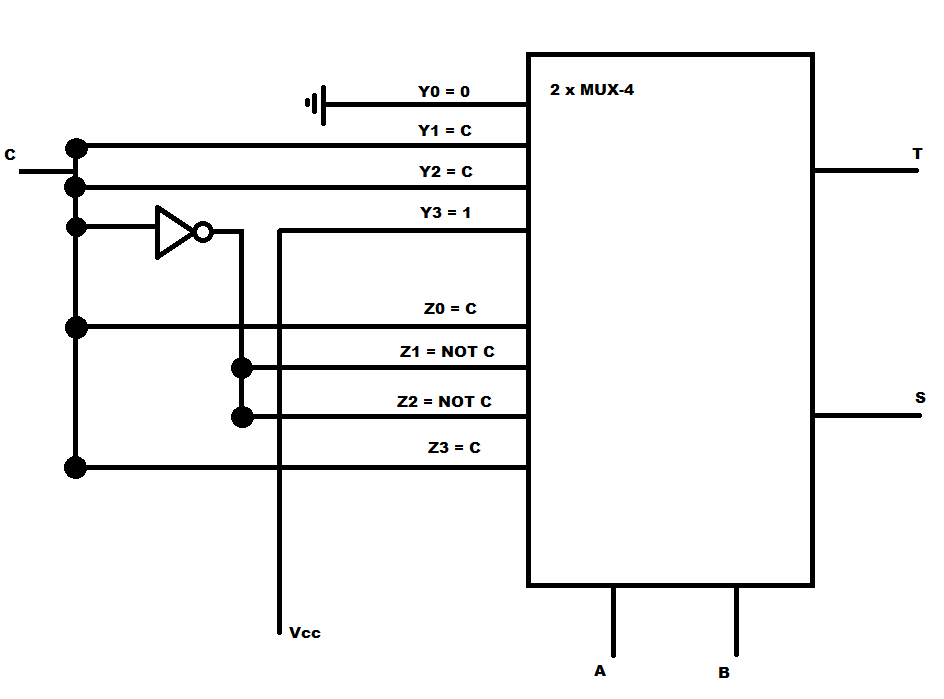
\includegraphics[width=.5\textwidth]{sc3e2s.png}
	\caption{Esquema de um somador completo com 3 entradas e 2 saídas montado com um Multiplexador}
	\label{fig:3e2s}
\end{figure}

O esquema apresentado acima foi montado com base na seguinte ideia: como A e B são as chaves seletoras, precisamos com que as entradas de dados, que terão seus dados selecionados, apresentem os resultados corretos em suas respectivas saídas. Portanto, para a saída T, temos:

\begin{figure}[H]
	\centering
	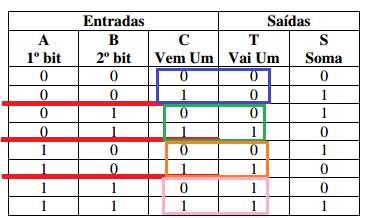
\includegraphics[width=.5\textwidth]{esparat.png}
	\caption{Entradas de dados para a saída T}
	\label{fig:est}
\end{figure}

Vemos que quando AB selecionar a entrada $Y_{0}$, ou seja, quando AB = 00, que T possui o valor 0 independente da entrada C. Portanto, temos que a entrada de dados $Y_{0}$ precisa apresentar esse valor para que quando AB for igual a 00 a saída apresente o valor correto de T. O mesmo ocorre para o caso em que AB = 11, porém, ao invés de T possuir o valor 0, ele possui o valor 1. Assim, conectando $Y_{0}$ na terra e $Y_{1}$ na fonte, conseguimos estes valores. Já para os casos em que AB = 01 e AB =10, vemos que a saída T tem que ser igual ao valor de C. Portanto, quando AB selecionar a entrada de dados $Y_{1}$ ou $Y_{2}$, a saída tem que possuir o valor de C. Portanto, conectamos C à essas entradas de dados.
Já para o caso da saída S temos a seguinte análise:

\begin{figure}[H]
	\centering
	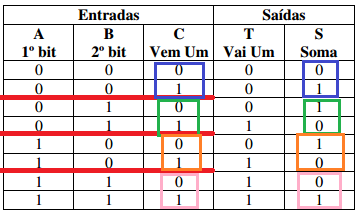
\includegraphics[width=.5\textwidth]{eds.png}
	\caption{Entradas de dados para a saída S}
	\label{fig:eds}
\end{figure}

Quando AB = 00 e AB = 11 temos que a saída S é a mesma que o valor da variável S. Portanto, ao selecionar as entradas de dados $Z_{0}$ e $Z_{3}$ precisamos que elas apresentem o valor de C, explicando a conexão feita. Quando AB = 01 e AB = 10, ocorre o oposto: a saída C possui o valor de NOT C. Portanto, temos que as entradas $Z_{1}$ e $Z_{2}$ precisam conter esse valor. 
Feito o esquema apresentado, o circuito foi montado e implementado com a ajuda dos materiais apresentados acima:

\subsection{Implementar uma função de 7 variáveis usando um multiplexador com 8 entradas de dados (MUX-8) construído com 2 multiplexadores com 4 entradas de dados (MUX-4 duplo)}

A função que foi implementada nesta parte do experimento é a seguinte:

$f(A,B,C,D,E,F,G) = FG + ABCD\overline{EF}G + \overline{ABCDEF}G + A\overline{B}CDEF\overline{G} + \overline{A}BCD\overline{E}F\overline{G} + ABCDE\overline{FG} + A\overline{BC}DE\overline{FG}$

Para implementar essa função com um decodificador e um multiplexador de 4 entradas de dados duplo, foi preciso usar o decodificador para gerar minitermos que serviriam como entrada de dados para o multiplexador. Como o decodificador possuía 4 entradas, as quatro variáveis mais significativas da função foram escolhidas para gerar os minitermos. Observando a função principal, temos que os minitermos gerados pelas quatro primeiras variáveis são:

$m_{0}=\overline{ABCD}$

$m_{7}=\overline{A}BCD$

$m_{9}=A\overline{BC}D$

$m_{11}=A\overline{B}CD$

$m_{15}=ABCD$

Portanto, temos que no esquema, o decodificador será da seguinte forma: 

\begin{figure}[H]
	\centering
	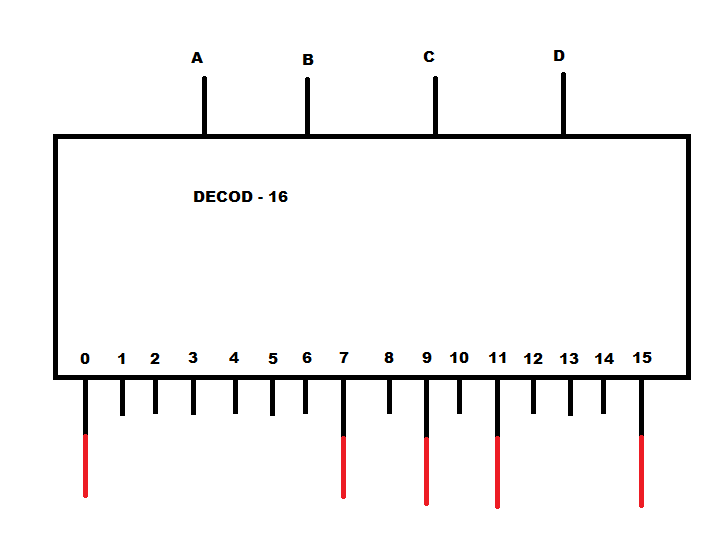
\includegraphics[width=.5\textwidth]{ed.png}
	\caption{Esquema do decodificador a ser implementado. Os fios em vermelhos são aqueles que apresentam os minitermos formados pelas variáveis mais significativas  que são válidos na função}
	\label{fig:edd}
\end{figure}

Antes de definir o que fazer com as saídas do decodificador é necessário primeiramente analisar as variáveis restantes. Fazendo esta análise na forma de tabela verdade, temos:


\section{Análise dos Resultados}
\label{sec:Resultados}

Faça uma análise crítica dos resultados obtidos nos experimentos. Esta análise pode ser feita item a item ou de uma forma geral.

Dica: Use pesquisa na Internet para tirar as dúvidas sobre edição em \LaTeX .

\section{Conclusão}
\label{sec:Conclusao}

A realização do experimento resultou num excelente aprendizado a respeito dos multiplexadores e demultiplexadores. Na experiência, os multiplexadores são tomados como circuitos combinacionais e a relação deles com os demultiplexadores também foi estudada.
Foi possível concluir que um multiplexador é uma ótima ferramenta para gerar funções booleanas. A simplificação de funções booleanas, como sempre, ajuda a simplificar o experimento, realçando novamente sua importância. A complexidade do experimento e o curto espaço de tempo que se tem para realiza-lo não permite atrasos de nenhum tipo e a simplificação das funções é de extrema ajuda nesse sentido

\newpage 
% Colocar aqui apenas as respostas dos itens da Auto-Avaliação
\section*{Auto-Avaliação}

\begin{enumerate}
    \item C
    \item C
    \item E
    \item C
    \item E
    \item C
    \item C
    \item C
    \item E
    \item E
    \item C
\end{enumerate}

\begin{table}[H]
	\centering
	\caption{Expected values of the obtained circuits' attributes.}
	\begin{tabular}{|c|c|c|c|c|c|c|c|}
		\cline{2-7}
		\multicolumn{1}{c}{} & \multicolumn{3}{|c|}{Phase 1} & \multicolumn{3}{c|}{Phase 2} & \multicolumn{1}{c}{} \\
		\hline
		Experiment & $n_g$ & $n_l$ & $n_t$ & $n_g$ & $n_l$ & $n_t$ & $t(s)$ \\
		\hline
		1 bit full adder & 8.16 & 3.8 & 47.6 & 5.03 & 3.0 & 25.93 & 99.13 \\
		2 bit full adder & 18.06 & 5.16 & 107.13 & 11.06 & 4.9 & 60.06 & 709.56 \\
		2 bit multiplier & 14.2 & 4.03 & 74.33 & 7.7 & 2.2 & 37.53 & 357.76 \\
		7 segment decoder & 47.53 & 5.83 & 270.46 & 32.86 & 5.0 & 176.4 & 740.63 \\
		Karnaugh 1 bit full adder & 19.0 & 6.0 & 102.0 & 5.03 & 3.0 & 24.8 & 130.73 \\
		\hline
	\end{tabular}
	\label{tab:resultados}
\end{table}
\end{document}
